\documentclass[A4paper]{article}
\usepackage[a4paper, total={7.2in, 10.5in}]{geometry}
\usepackage{tikz}
\usetikzlibrary{calc}
\usepackage{setspace}
\usepackage{graphicx}
\usepackage{amsmath}
\usepackage{pgfplots}
\usepackage[hidelinks]{hyperref}
\usepackage{bookmark}
\DeclareMathOperator\cosec{cosec}

\graphicspath{ {./images/} }

\setlength{\parindent}{0pt}

\title{A Level Mathematics - Mechanics}
\author{Xingzhi Lu (2129570@concordcollege.org.uk)}
\date{2024}

\begin{document}
	\maketitle

	\section{Vectors}
	\subsection{Calculations}
	\begin{itemize}
		\item $\vec{a}=\vec{a_x}+\vec{a_y}$
		\item $|\vec{a_x}|=|\vec{a}|\cos\theta$
		\item $|\vec{a_y}|=|\vec{a}|\sin\theta$
		\item $\tan\theta = \dfrac{|\vec{a_y}|}{|\vec{a_x}|}$
		\item $|\vec{a}|^2=|\vec{a_x}|^2+|\vec{a_y}|^2$
		\item $\vec{a} \cdot \vec{b} = |\vec{a}||\vec{b}|\cos\theta = x_1x_2+y_1y_2$
		\begin{description}
			\item If $a\perp b$: $\vec{a} \cdot \vec{b} = 0$
		\end{description}
		\item $\cos \theta = \dfrac{\vec{a} \cdot \vec{b}}{|\vec{a}||\vec{b}|}$
		\item $\text{Unit vector (magnitude = 1)} = \dfrac{\vec{a}}{|\vec{a}|}$

	\end{itemize}
	\subsection{Find the resultant of two vectors}
	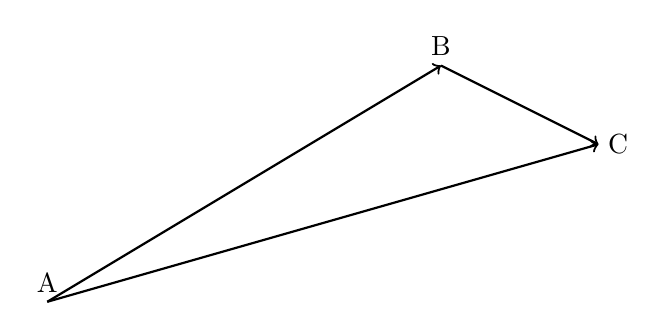
\begin{tikzpicture}
		\draw[->,thick] (0,0) -- (5,3);
		\draw[->,thick] (5,3) -- (7,2);
		\draw[->,thick] (0,0) -- (7,2);
		\node[above] at (0,0) {A};
		\node[above] at (5,3) {B};
		\node[right] at (7,2) {C};
	\end{tikzpicture}\\
	\\
	$\overrightarrow{AC}=\overrightarrow{AB}+\overrightarrow{BC}$\\
	$|\overrightarrow{AC}|$ can be found by sine or cosine rule

	\pagebreak

	\section{Forces and motion}
	
	\subsection{Types of motion}
	
	\subsubsection{Constant speed motion}
	\textbf{Calculations:}
	\begin{itemize}
		\item $v$ is constant, $a=0$
		\item $d=vt$
	\end{itemize}
	\textbf{Motion graphs:}\\
	%d-t graph
	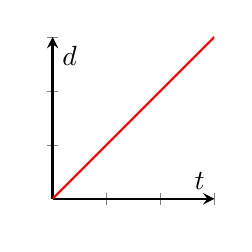
\begin{tikzpicture}
		\begin{axis}[
			xmin = 0, xmax = 30,
			ymin = 0, ymax = 30, axis lines=center, axis line style={thick},
			width=0.3\textwidth, height=0.3\textwidth,
			xlabel=$t$,ylabel=$d$,
			yticklabel=\empty, xticklabel=\empty]
			\addplot[
			domain = 0:30,
			samples = 200,
			smooth,
			thick,
			red,
			] {x};
		\end{axis}
	\end{tikzpicture}
	%v-t graph
	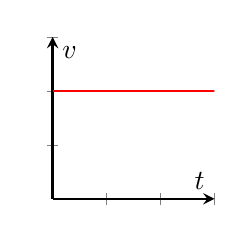
\begin{tikzpicture}
		\begin{axis}[
			xmin = 0, xmax = 30,
			ymin = 0, ymax = 30, axis lines=center, axis line style={thick},
			width=0.3\textwidth, height=0.3\textwidth,
			xlabel=$t$,ylabel=$v$,
			yticklabel=\empty, xticklabel=\empty]
			\addplot[
			domain = 0:30,
			samples = 200,
			smooth,
			thick,
			red,
			] {20};
		\end{axis}
	\end{tikzpicture}
	%a-t graph
	\begin{tikzpicture}
		\begin{axis}[
			xmin = 0, xmax = 30,
			ymin = 0, ymax = 30, axis lines=center, axis line style={thick},
			width=0.3\textwidth, height=0.3\textwidth,
			xlabel=$t$,ylabel=$a$,
			yticklabel=\empty, xticklabel=\empty]
			\addplot[
			domain = 0:30,
			samples = 200,
			smooth,
			thick,
			red,
			] {0};
		\end{axis}
	\end{tikzpicture}
	
	
	\subsubsection{Uniform acceleration motion}
	\textbf{Calculations:}
	\begin{itemize}
		\item $d=v_it+\dfrac{1}{2}at^2$
		\item $v_f=v_i+at$
		\item $v_f^2=v_i^2=2as$
		\item $d=\overline{v}t$
		\item $\overline{v} = \dfrac{v_i+v_f}{2}$
	\end{itemize}

	\subsubsection{Free fall}
	Air resistance is ignored, so $a=g$\\
	\textbf{Calculations:}
	\begin{itemize}
		\item $v_i = 0$
		\item $v_f = gt$
		\item $h=\dfrac{1}{2}gt^2$
	\end{itemize}
	\subsubsection{Vertically upward}
	\textbf{Calculations:}
	\begin{itemize}
		\item $v = u - gt$
	\end{itemize}
	Rising and falling at the same height: speed same, opposite direction
	\subsubsection{Projectile}
	\textbf{Calculations:}
	\begin{itemize}
		\item $y=\tan\theta x - \dfrac{g}{2u^2}(1+\tan^2\theta)x^2$
		\item range = $\dfrac{u^2\sin 2\theta}{g}$
		\item greatest height: $\dfrac{u^2\sin^2\theta}{2g}$
		\item Time to flight (back to x-axis) = $\dfrac{2u\sin\theta}{g}$
		\item Time to greatest height: $\dfrac{u\sin\theta}{g}$
	\end{itemize}
	\subsection{Types of forces}
	\begin{description}
		\item[Weight: ] $W=mg$
		\item[Normal contact force: ] symbol = $R$ or $N$
		\item[Static friction: ] Depends on driving force, $F\leq \mu R$
		\item[Dynamic friction: ] $f=\mu R$ ($\mu$=coefficient of kinetic friction)
		\item[Tension: ] $T=\text{elastic coefficient}\times\text{extension}=k\times\Delta x$
	\end{description}
	
	\subsection{Common scenarios}
	\subsubsection{Lift}
	\begin{description}
		\item[Rising: ] $R-W=ma$
		\item[Moving down: ] $W-R=ma$
		\item[On rest: ] $R=W$
	\end{description}
	
	\subsubsection{Slope}
	\begin{itemize}
		\item Coordinate: centre = object, x-axis = slope surface, y-axis = perpendicular to slope surface
		\item Calculate resultant force in $x$ and $y$ direction
		\item Use SUVAT equations to find distance / speed / time
	\end{itemize}
	
	\subsubsection{One whole system}
	e.g. on a train / car
	\begin{itemize}
		\item Acceleration is the same across the whole system
		\item Internal force can be ignored
		\item Tension at the same rope has the same magnitude
	\end{itemize}
	
	\subsubsection{Fixed pulley}
	\begin{itemize}
		\item Same tension
		\item Same magnitude for acceleration (different direction)
		\item Use simultaneous equations to find tension
	\end{itemize}
	
	\pagebreak

	\section{Momentum}
	\subsection{Definitions}
	\begin{itemize}
		\item $p=mv$
		\item $\Delta p = m\Delta v = m a t = Ft$
		\item Impulse = $Ft=\delta p = m(v_f-v_i)$
	\end{itemize}
	
	\subsection{Collision}
	\begin{description}
		\item[Elastic: ] KE conserved
		\item[Inelastic: ] KE not conserved
	\end{description}

	\pagebreak


	\section{Moments}
	\subsection{Definition}
	\textbf{Turning} effect of the force on a rigid body.\\
	Clockwise moment of $F$ about P: $|F|\times d= \vec{F}\times\vec{d} = |F||d|\sin\theta$
	\subsection{Right hand rule}
	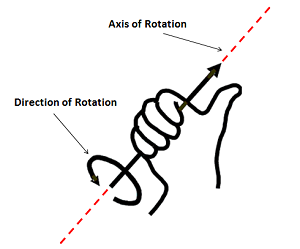
\includegraphics[width=0.4\textwidth]{rhr}\\
	$\vec{a} \times \vec{b}$= from $\vec{a}$ to $\vec{b}$\\
	$\vec{b} \times \vec{a}$= from $\vec{b}$ to $\vec{a}$
	
	\subsection{Tilting about a pivot}
	Support / tension force at any point = 0
	

	\pagebreak

	\section{Common questions}
	\subsection{Projectile}
	\subsubsection{Asking for improvements}
	\begin{itemize}
		\item Ball modelled as particle / no volume
		\item Air resistance ignored
		\item Ball doesn't spin / spin ignored
	\end{itemize}
	\subsection{Moment}
	\subsubsection{Plank modelling}
	\begin{description}
		\item[Modelled as rod: ] Plank remains straight
		\item[Mass modelled as particles: ] Weights act at the ends of plank
	\end{description}
	
	
	
	

\end{document}